%% This is an example first chapter.  You should put chapter/appendix that you
%% write into a separate file, and add a line \include{yourfilename} to
%% main.tex, where `yourfilename.tex' is the name of the chapter/appendix file.
%% You can process specific files by typing their names in at the 
%% \files=
%% prompt when you run the file main.tex through LaTeX.
\chapter{Introduction}

	
A 3D scanner is a combination of hardware and software components used for acquisition of three dimensional information from a scene.  Recent applications[1] of 3D scanners seems to suggest that they are not only used for metric reconstructions but also for acquiring information regarding relative placement of objects in 3D space which do not essentially requires metric information,  examples are \textit{affine} and \textit{projective} reconstructions[2],[3], example application includes robotic navigation where 3D coordinates in terms of physical units are not required but only a non-metric 3D information suffices[4], whereas the \textit{euclidean} reconstruction comes under category of metric reconstruction and is also the subject of this work.\newline


3D scanners find applications in robotic controls for example a laser scanner can act like an eye for robot, in site modeling and lay-outing, establishing benchmark for preexisting shape/state for studying structural changes in response to extreme environmental conditions, to create Geometric information systems, it is also used for sub-surface scanning in mines. Of course in entertainment where currently Microsoft Kinect is a leading example. It is also used in reverse-engineering a mechanical component which requires a precise digital model of object. In cultural heritage preservation, where Michelangelo, Monticello, Kasubi-tombs etc are prime examples. It is also used in Medical CAD/CAM for example to produce orthosis, prosthesis and dental implants. In industrial quality inspection and meteorology it is used for measuring geometric dimension accuracy, automation of quality assurance process for example in assembling a car it must be ensured that geometry of individual components is accurate so that it can fit together for reliable operation.\newline 


Although recent work on Monocular 3D[5] has lead to development of methods which can extract approximate three dimensional  information even from single view using cues like perspective distortion, boundary shades, shadow, occlusion etc, exact metric reconstruction still requires at least 2 views. In simplest case with 2 views, there is a need to recover a relationship between these views so as to compute depth of a point common to both views with respect to a global coordinate system. But since depth is to be interpreted and utilized for real world practical applications(as is the case with this work) it has to be expressed in terms of physical units like `mm', `cm', `feet' etc. \newline


So clearly above discussion point towards three major problems associated with 3D metric reconstruction:Correspondence between views,  Calibration of viewing elements to determine the relation between abstract world of these elements(in our case these elements are projector and camera) and  our physical world, and computation of depth given correspondence and calibration information.  Specifically for 3D reconstruction, first system is calibrated, then correspondence between camera and projector is calculated, and then using the calibration and correspondence information triangulation is performed to compute 3D coordinates of point in real world with respect to a reference coordinate system. 
 
\section{Motivations for development and accuracy analysis of 3D scanner} 
Motivation for this work comes from the fact that as per our current knowledge there is no development expertise in the field of 3D scanners based on structured-light technique in our country. This approach provides high accuracy, portability, low-cost solution to dimension measurement and reverse-engineering applications. Although measurement accuracy of these systems is still lower than CMM machines, it can be expected to be achievable with high quality camera and projector optics and improvements in measurement algorithm. 
Furthermore current commercial scanners using structured-light technique are considerably more costlier for example[6] where even cost of 3D scanner software is >1.5 Lakhs which excludes  cost of hardware components. Hence our development work can provide a low-cost alternative to these systems.\newline 


Specifically, in CDM,BARC we have a CMM machine [Zeiss UPMC-850] for dimensional inspection of fabricated job which is reported to have accuracy of $4\mu m$ within measurement volume of 850mm X 1200mm X 600 mm. But dimension measurement time for complex jobs, strict temperature requirements to maintain acceptable sphere-form of Ruby balls used in probes, lack of portability of measuring device, higher power consumption for maintaining near frictionless air-bearings and a certain operating temperature and larger space requirements are motivating factors for this work. In addition, in B.A.R.C Hospital we have a common requirement of producing artificial teeth for implantation but an expertise is needed to deal with its technical details. Furthermore Computer Division is working on CFD simulation problem in collaboration with IIT-Guwahati where a digitized model of a physical object will be more insightful to use instead of using an artificial object with ideal/perfect dimensions, further development of our work can provide 360 degree 3D scans of an object which can be used in such simulations. 
 
 
 
\section{Scope of this work} 
Scope of the work is limited to development of a 3D dimension measurement system based on Coded-phase shift technique. Further, tests are devised to assess accuracy of individual components of the system developed. Specifically, the effect of non-linearity of output response of projector(characterized by \textit{gamma value}) on accuracy of stereo-correspondence is studied. In addition, the effect of increasing the number of phase-shifted patterns on accuracy of stereo-correspondence has also been studied as it has been both theoretically and practically demonstrated in the literature[7] that increasing the number of phase shifted patterns reduces the effect of non-linearity of projector output response and hence increases accuracy of estimated stereo-correspondence. Here i have tested these claims for 3, 4 and 5 phase-shifted sinusoidal fringe patterns. Similarly, tests to assess accuracy of system calibration parameters are performed. To evaluate accuracy of complete 3D scanning pipeline, a comparative evaluation of measurement accuracy and precision of developed system with nowadays commonly available 3D sensor \textit{Microsoft Kinect} is performed. However during development and performance assessments of developed system, shortcomings of techniques used for both development and accuracy assessments were observed which are reported in chapter-6 of this thesis which may pave the way for our future work.  
 
\section{Structure of thesis} 
Chapter-2 describes the currently most popularly used approaches for solving system calibration problem. It further describes the development and working of system calibration module. Chapter-3 reviews the current state of approaches to solve stereo-correspondence problem and further describes the development and working of Coded phase-shift scanning technique. Chapter-4 first reviews the current approaches to solve the triangulation problem and then describes the approach used in this work. Chapter-5 explains the experiments performed to assess accuracy of modules within the scope of this work namely stereo-correspondence and system calibration modules. It further describes the work done for comparative evaluation of measurement accuracy and precision of Coded-phase-shift scanner and Microsoft Kinect. In chapter-6 conclusions emerging from this work are described and directions for future work are proposed. Finally, Bibliography concludes the thesis.  
 
 
 
  
\section{Principle of operation and graphical layout of the developed system} 
Solving stereo-correspondence problem amounts to providing unique relation between points of camera and projector such that related camera and projector points will be 2D projections of same point in real 3D world. Coded phase-shift technique being a structured light technique solves this problem by assigning unique code to each point(theoretically) in the 3D scene. Specifically, this technique involves projection of sinusoidal phase-shifted patterns(which assigns unique phase value to each projector pixel within a sinusoidal period) followed by binary-coded patterns (which assign unique period number to each sinusoidal fringe period) onto object to assign unique phase-value to each point in the scene. Camera captures these patterns and computes the phase of incident signal at each pixel(which indirectly assigns phase to the pixel). Correspondence problem is then solved by determining the camera-projector pixel pair having same phase value.\newline  


Sinusoidal and binary-coded patterns are generated by \textit{\textbf{Pattern generator module}}. Camera captures the projected patterns through \textit{\textbf{Pattern projection and capture module}} and for each pixel, phase of the original incident signal is computed through \textit{\textbf{Phase wrapper and Phase unwrapper modules}}. This phase value at each pixel relates a camera pixel to the corresponding projector pixel which are seeing a common point in the real 3D world through \textit{\textbf{Absolute phase computation module}}. Further the calibration parameters for camera, projector and relative orientation and position of camera with respect to projector are estimated by \textit{\textbf{System calibration module}}. Once the system calibration parameters and stereo-correspondence information is known, triangulation can be applied through \textit{\textbf{Triangulation module}}. Figure~\ref{fig:correspond_triangulate} shows the optical triangulation process.\newline 
\begin{figure}[!h]
\centering
\begin{tikzpicture}
\pgftext{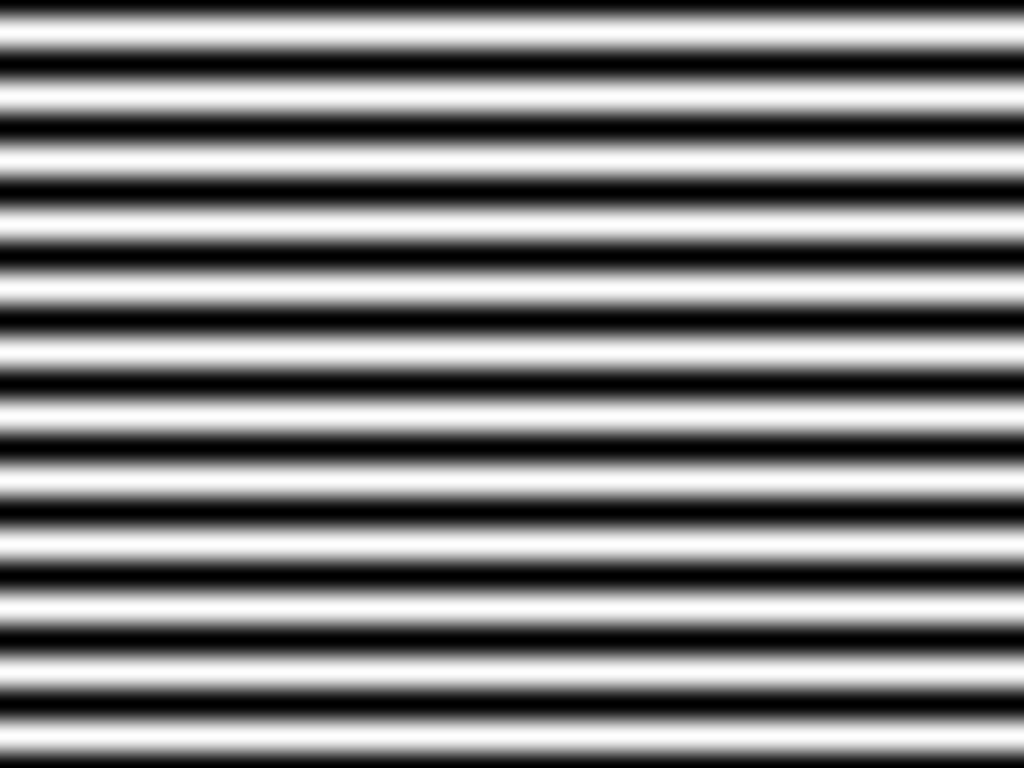
\includegraphics[width=5cm,height=5cm]{../img_source/phase_hor_1.jpg}}
\node at (0.0,-3) {\color{red} Projector image};
\pgftext[at=\pgfpoint{6cm}{0cm}]{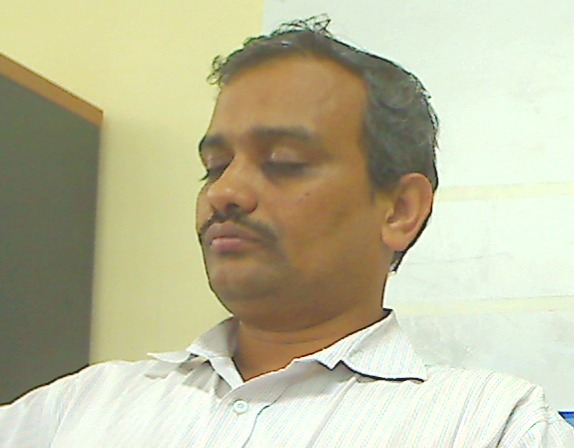
\includegraphics[width=5cm,height=5cm]{../img_source/face_2d.jpg}}
\node at (6,-3){\color{red} Camera image};
\pgftext[at=\pgfpoint{3cm}{9cm}]{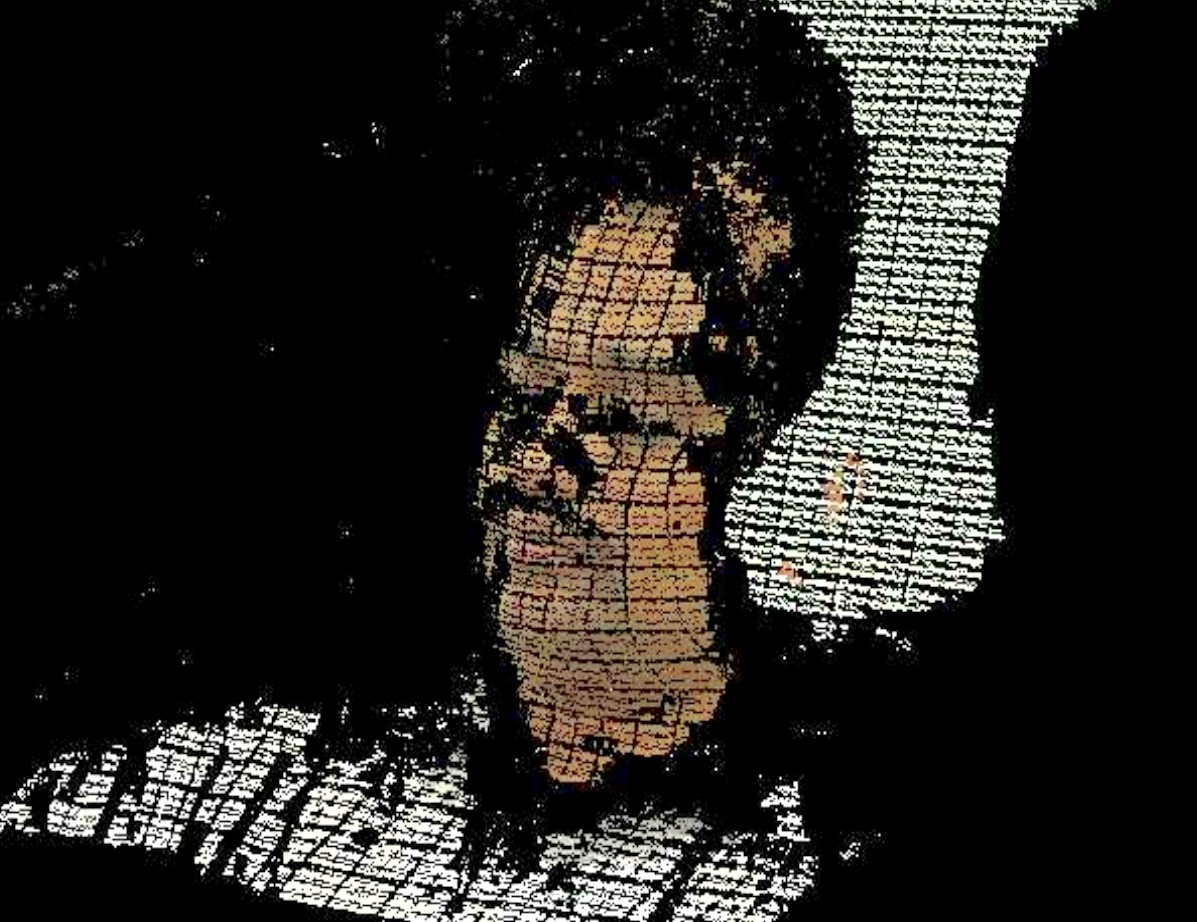
\includegraphics[width=5cm,height=5cm]{../img_source/face_3d.jpg}}
\node at (3,12){\color{red} Real-world object};
\draw [->](0,0)--(3.2,8);
\draw [->](3.2,8)--(6.1,-.7);
\draw[.] (6,0);
\fill [green] (3.2,8) circle[radius=2pt];
\fill [green] (6.1,-.7) circle[radius=2pt];
\fill [green] (0.0,0.0) circle[radius=2pt];
\end{tikzpicture}
\caption{Stereo correspondence and triangulation}
\label{fig:correspond_triangulate}
\end{figure}
\FloatBarrier
In figure~\ref{fig:correspond_triangulate}, a point in \textit{Projector image} is related to a point in \textit{Camera image} because they are 2D projections of a common point in the scene using the estimated stereo-correspondence. Once system is calibrated, ray-ray intersection between optical ray of camera and that of corresponding projector pixel gives the (X,Y,Z) coordinates of real-world point in \textit{physical unit} like `mm', `m' etc. \newline

\indent Figure~\ref{fig:arch} graphically represents the layout of our 3D scanner system, which can be referred during thesis. Working of \textbf{\textit{System calibration module}} is documented in chapter-2. \textbf{\textit{Pattern generation, Pattern projection and capture, Phase wrapper, Phase unwrapper, Absolute phase computation modules}} are explained in chapter-3. \textbf{\textit{Triangulation module}} has been described in chapter-4. 

\begin{figure}[!h]
\centering
\begin{tikzpicture}
  [node distance=2.0cm,
  start chain=going below,]
     \node[punktchain, join] (intro) {Pattern generation};
     \node[punktchain, join] (probf)      {Pattern projection and capture};
     \node[punktchain, join] (investeringer)      {Phase wrapping};
     \node[punktchain, join] (perfekt) {Phase unwrapping};
     \node[punktchain,join] (emperi) {Absolute phase computation};
\node[punktchain,join](triangulate){\textbf{\textit{Triangulation}}};
\begin{scope}[start branch=x,every join/.style={->,thick,shorten <=1pt},]
\node[punktchain,on chain=going left,join=by {<-},node distance=-14.0cm](calib) {\textbf{\textit{System calibration}}};
\end{scope}

\draw[tuborg, decoration={brace}] let 
  \p1=(intro.north), \p2=(emperi.south) in 
   ($(2.3, \y1)$) -- ($(2.3,\y2)$) node[tubnode] {\textbf{\textit{Stereo correspondence}}};

\node at (-1.8,-1.5) {\textit{Generated patterns}};

\node at (-1.7,-4.8){\textit{Captured patterns}};

\node at (-1.5,-8.1){\textit{Wrapped phase}};

\node at (-1.7,-11.4){\textit{Unwrapped phase}};

\node at (-3.1,-14.7){\textit{Camera-projector correspondence}};

\node[above] at (4.5,-16.5){\textit{camera,projector}}; 
\node[below] at (4.6,-16.4){\textit{calibration parameters}};
\end{tikzpicture}
\caption{Architecture of the developed system}
\label{fig:arch}
\end{figure}


